\subsection{Generation}  \label{sec:Generation}
\subsubsection{\textbf{Definition}}
Personalized generation incorporates user-specific retrieved documents $D^*$, task-specific prompt $prompt$, and user preference information $p$ via the generator $\mathcal{G}$ parameterized by $\theta$ to produce tailored content $g^*$ aligned with individual preference, where the flow is shown in Figure~\ref{fig:generation}. The generation process can be formulated as
\begin{equation}
g^* = \mathcal{G} \left(D^*,\text{prompt},p,\theta \right) .
\end{equation}
Personalized generation can be achieved by incorporating explicit and implicit preferences. Explicit preference-driven methodologies utilize direct input signals (\eg $D^*$, $\text{prompt}$, and $p$), to tailor outputs to specific user preferences. Conversely, implicit preference-encoded approaches embed personalized information within the parameters $\theta$ of the generator model, during training, thereby facilitating preference alignment without the necessity for explicit runtime inputs.

\begin{figure}[t]
    \centering
    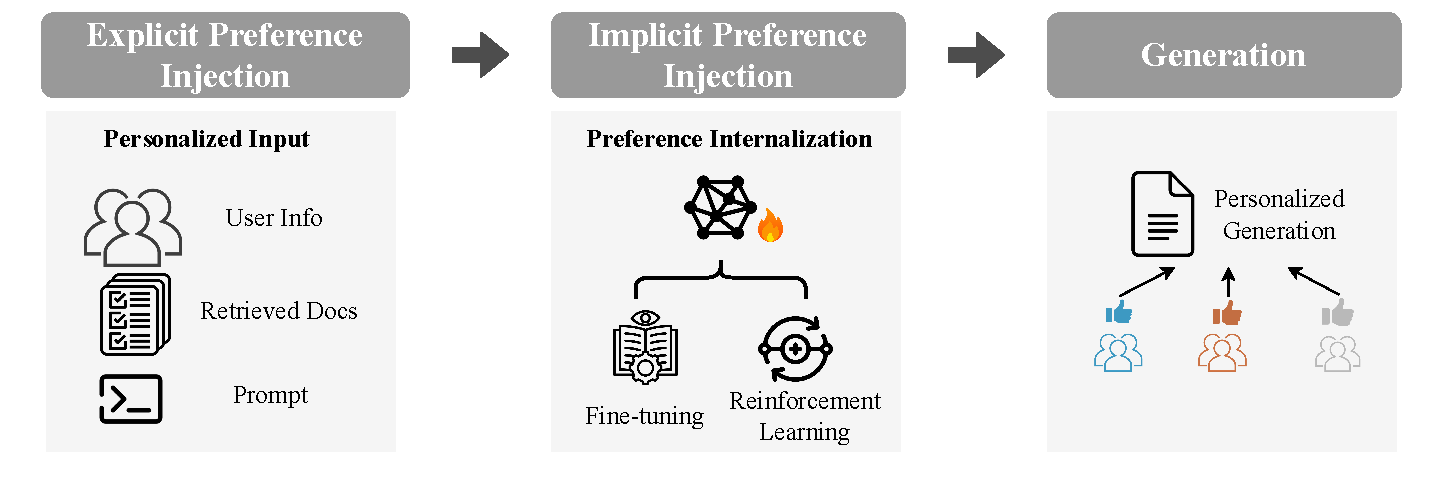
\includegraphics[width=\linewidth]{figures/generation.pdf}
    \caption{Overview of the personalized generation stage.}
    \label{fig:generation}
\end{figure}

\subsubsection{\textbf{Generation from Explicit Preferences}}
Integrating explicit preferences into LLMs facilitates personalized content generation. Explicit preference information encompasses user demographic information (\eg age, occupation, gender, location), user behavior sequences (reflecting historical behavioral patterns), and user historical output texts (capturing writing style and tone preferences). The injection of explicit preferences for personalized generation can be categorized into three types: (1) Direct-integrated Prompting, (2) Summary-augmented Prompting, and (3) Adaptive Prompting.

\paragraph{\textbf{\textit{{(1). Direct-integrated Prompting.}}}}
Integrating user explicit preferences into language models through prompting enables the prediction of users' intent and behavioral patterns, facilitating personalized content generation. For instance, P$^2$~\cite{jiang2023evaluating}, Character Profiling~\cite{yuan2024evaluating}, and OpinionQA~\cite{santurkar2023whose} integrate personalized data into LLMs through prompting for role-playing task, thereby aligning the model's responses with specified user profiles. ~\citet{kang2023llms} and ~\citet{liu2023chatgpt} integrate interaction histories into LLMs via prompting to predict user rating for candidate items. Cue-CoT~\cite{wang2023cue} employs chain-of-thought reasoning to infer user needs from contextual cues, enabling personalized responses to in-depth dialogue questions. Additionally, TICL~\cite{cho2025tuning} proposes a trial-and-error framework that critiques initial LLM-generated responses, derives explanations and integrates these negative examples into prompts to improve personalization alignment.

\paragraph{\textbf{\textit{{(2). Summary-augmented Prompting.}}}}
Direct integration of personalized information via prompting struggles with ambiguous intent signals: Lengthy interaction histories introduce noise that obscures critical behavioral patterns~\cite{liu2024lost}, while sparse behavioral data lacks sufficient context for LLMs to derive meaningful user preferences. To address these issues, recent approaches focus on summarizing user personalized intents and integrating them into prompts. For instance, GPG~\cite{zhang2024guided} extracts key user habits and preferences from personal contexts, enabling fine-grained personalization. Similarly, LLMs are employed to generate task-specific summaries of user preferences, enhancing retrieval-augmented personalized generation capabilities~\cite{richardson2023integrating}. In recommendation systems, ONCE~\cite{liu2024once}, LLMTreeRec~\cite{zhang2025llmtreerec}, and KAR~\cite{xi2024towards} leverage historical user-item interactions to summarize user preferences. Furthermore, Matryoshka~\cite{li2024matryoshka} generates user preference summaries by dynamically retrieving and synthesizing historical data.

\paragraph{\textbf{\textit{{(3). Adaptive Prompting.}}}}
Manually designing personalized prompts demands both expert knowledge and significant labor, motivating the development of automated methods for personalized prompt generation. For example, \citet{li2024learning} trains a personalized prompt rewriter via supervised and reinforcement learning. RecGPT~\cite{zhang2024recgpt} and PEPLER-D~\cite{li2023personalized} leverage prompt tuning to generate personalized prompts, enhancing sequential and explainable recommendations, respectively. GRAPA~\cite{qu2024graph} integrates semantic and collaborative signals from user-item interaction graphs with graph neural networks to generate context-aware personalized prompts. SGPT~\cite{deng2024unlocking} employs prompt tuning
to jointly model common and group-specific patterns, bridging generalized and personalized federated learning paradigms. Furthermore, PFCL~\cite{yu2024personalized} achieves multi-granularity human preference modeling: coarse-grained prompts distill shared knowledge, while fine-grained prompts adapt to individual user characteristics.

\subsubsection{\textbf{Generation from Implicit Preferences}}
Unlike explicit preference modeling, which captures user preferences through textual input, implicit preference-based methods incorporate personalization through internal parameters. This personalization is achieved either through Parameter-Efficient Fine-tuning (PEFT) techniques, such as LoRA~\cite{hu2022lora}, or reinforcement learning-based approaches for preference alignment~\cite{li2024learning,chen2024pad}. Based on these strategies, we classify existing methods into two categories: (1) Fine-tuning-Based Methods and (2) Reinforcement Learning-Based Methods.

\paragraph{\textbf{\textit{{(1). Fine-tuning Based Methods.}}}}
For fine-tuning methods, LoRA is the most widely adopted since it is resource-efficient and enables rapid adaptation without compromising model performance. PLoRA~\cite{zhang2024personalized} introduces a personalized knowledge integration framework that combines task-specific LoRA with user-specific knowledge. Similarly, LM-P~\cite{wozniak2024personalized} personalizes information via LoRA by incorporating User ID as a personalization factor. MiLP~\cite{zhang2024personalized} employs Bayesian optimization to determine the optimal personalization injection configuration, including LoRA settings, to effectively capture and utilize user-specific information. OPPU~\cite{tan2025democratizing} and PER-PCS~\cite{tan2024personalized} follow a similar approach, leveraging user history data for fine-tuning LoRA-based personalization. However, PER-PCS differs by incorporating a gating module that selects the appropriate LoRA, enabling fine-grained personalization. Additionally, Review-LLM~\cite{peng2024reviewllm} integrates LoRA for supervised fine-tuning in the task of personalized review generation.

Beyond LoRA-based approaches, alternative pipelines have been proposed for personalized generation. UserIdentifier~\cite{mireshghallah2021useridentifier} introduces a user-specific identifier, significantly reducing training costs while enhancing personalized demonstration. UserAdapter~\cite{zhong2021useradapter} proposes user-independent prefix embeddings, leveraging prefix tuning for personalization. Meanwhile, HYDRA~\cite{zhuang2406hydra} achieves implicit personalization by training user-specific headers. Recently, researchers have also explored fine-tuning personalized model on edge devices~\cite{peng2024pocketllm} and collaborative learning between small and large language models to enable more personalized generation~\cite{zhang2024cogenesis}.

\paragraph{\textbf{\textit{{(2). Reinforcement Learning Based Methods.}}}}
Apart from fine-tuning based methods, recent research has explored reinforcement learning based techniques to personalize text generation by aligning outputs with user preferences. P-RLHF~\cite{li2024personalized} has been proposed to jointly learn a user-specific and reward model to enable text generation that aligns with a user's styles or criteria. P-SOUPS~\cite{jang2023personalized} models multiple user preferences as a Multi-Objective Reinforcement Learning (MORL) problem, decomposing preferences into multiple dimensions, each trained independently. PAD~\cite{chen2024pad} aligns text generation with human preferences during inference by utilizing token-level personalized rewards to guide the decoding process. REST-PG~\cite{salemi2025reasoning} introduces a framework that trains large language models to reason over personal data during response generation. This approach first generates reasoning paths to enhance the LLM's reasoning ability and then employs Expectation-Maximization Reinforced Self-Training to iteratively refine the model based on its high-reward outputs. Additionally,~\citet{salemi2024optimization} incorporate reinforcement learning into the RAG pipeline to improve retrieval accuracy, thereby enhancing the personalization of generated content. Other applications include RewriterSlRl~\cite{li2024learning}, which has been introduced to generate text via RL-based personalized prompt rewriting using API-based LLMs, and ~\citet{kulkarni2024reinforcement}, who explore the use of reinforcement learning to optimize RAG for improving the relevance and coherence of chatbot responses in specialized domains, ultimately enhancing user satisfaction and engagement.

\subsubsection{\textbf{Discussion}}
Personalized generation can be adopted via both explicit and implicit preference injection, yet they exhibit distinct characteristics that make them suitable for different scenarios.
In explicit preference-based generation, personalization is clearly defined through user profile descriptions, contextual information, and similar inputs, which are incorporated into generators via prompts. A key advantage of this approach is explainability, as the personalized information is explicitly provided and easily traceable. 
Despite leveraging provided preferences and internal knowledge, explicit preference injection's personalization is constrained by model capabilities and irrelevant information interference.
In contrast, implicit preference-based generation internalizes personalized information into the generator's parameters through scene-specific personalized data, thereby adapting the model for more fine-grained personalization. However, these methods typically incur substantial training and computational costs, as they require fine-tuning the generator’s internal parameters. Therefore, selecting between these approaches should be guided by the specific application scenario and resource constraints.